%!TEX root = AllegThesis.tex
%
% $Id: ch04_implementation.tex
%
\chapter{Energy Reconstruction}\label{ch:implem}

In this chapter we present methods for reconstructing the energies deposited by particles using ADC waveform measurements. This analysis is key for differentiating electrons from sources of background, most notably protons.

\section{Methodology}

\begin{figure}[htp!]
    \centering
    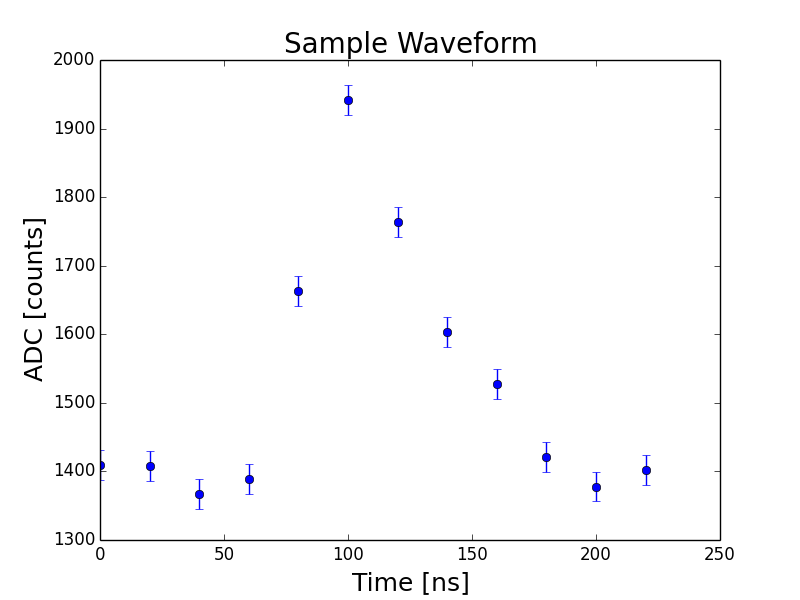
\includegraphics[scale=0.5]{Images2/sampleWaveform.png}
    \caption{Sample waveform of ADC output.}
    \label{fig:sampleWaveform}
\end{figure} 
To develop the following methods, 500 events of conversion electrons with full hit background overlay (accidental signals resulting from unavoidable processes related to stopping muons in aluminum) were simulated using Mu2e Offline. This provides the most accurate simulations of the output of the ADCs to date. Each hit is recorded as a 240 ns interval of output from the ADC. Samples are measured at a fixed clock frequency of 50 MHz. Hence, twelve samples are measured for a given hit. Using a 12-bit ADC, each sample lies in the range of 0 to 4095 counts. Four of these samples, called presamples, are measured immediately prior to the signal crossing threshold. A sample waveform is shown in Figure \ref{fig:sampleWaveform}. 


\subsection{Monte Carlo Truth Energy}
For comparison, a variable provided in the Mu2e simulations, known as the Monte Carlo truth energy (MC energy) has been used. The MC energy is defined to be the total energy deposited on a straw over the interval of a given hit. In many cases the MC energy describes precisely the value we hope to compute. However, for a small portion of cases in which two or more particles go through the straw within the same 240 ns period, this value will be higher than the computed energy of a hit. A frequency plot of the MC energies of the electrons and protons is shown in Figure \ref{mcenergydistributions}. Electron hits can be separated by cutting on the deposited energy. Note that for any cut in energy, it will be impossible to completely differentiate protons and electrons due to the overlap in energies.

\begin{figure}[htp!]
    \centering
    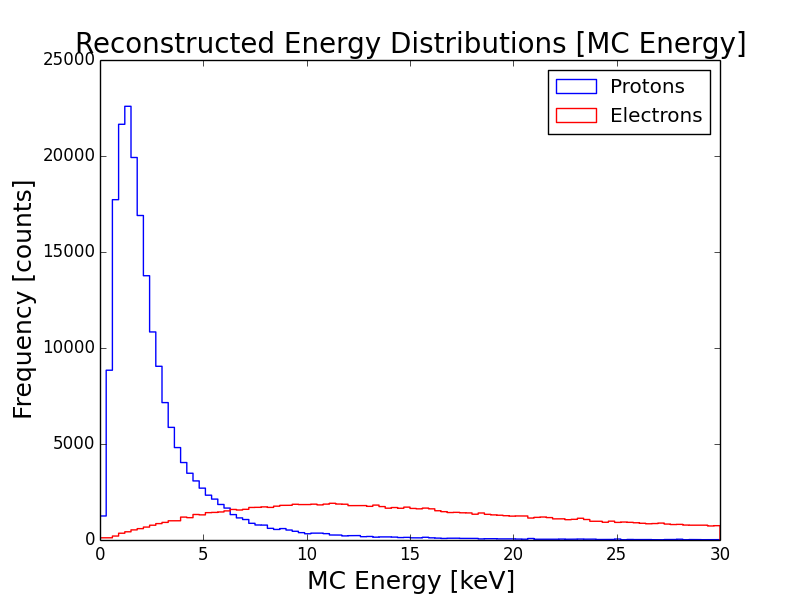
\includegraphics[width=0.6\textwidth]{Images2/mcenergy.png}
    \caption{MC energy frequency distributions for electrons and protons.}
    \label{mcenergydistributions}
\end{figure} 


\subsection{Sum Method}

The current method in the Mu2e software used to compute the energy of a hit is to simply sum the values of the ADC and subtract the mean of the presamples. This method has already been succesfully implemented in the Mu2e simulations and can therefore be considered the baseline method. In other words, the method developed over the following sections must differentiate protons and electron hits at least as well as the sum method.


\subsubsection{Methods of Comparison}
To compare the various methods, a purity-efficiency plot is used. For any method, the purity-efficiency plot contains a comparison between the power of rejection of protons and the acceptance rate of electrons for various cuts in energy. For example, the purity-efficiency curves for the sum method and MC energy data are shown in Figure \ref{rejectionPlotSumAndMCenergy}. Conceptually, it is easy to see that a "better" method's rejection curve will lie above the purity-efficiency curve of a "poorer" method. Therefore, this type of plot will be used as the main tool in comparing the success of different methods. %In addition, since there is a gap betwen the two curves, this comparison shows that improvement over the sum method is possible.

\begin{figure*}[ht!]
    \centering
    \makebox[0pt]{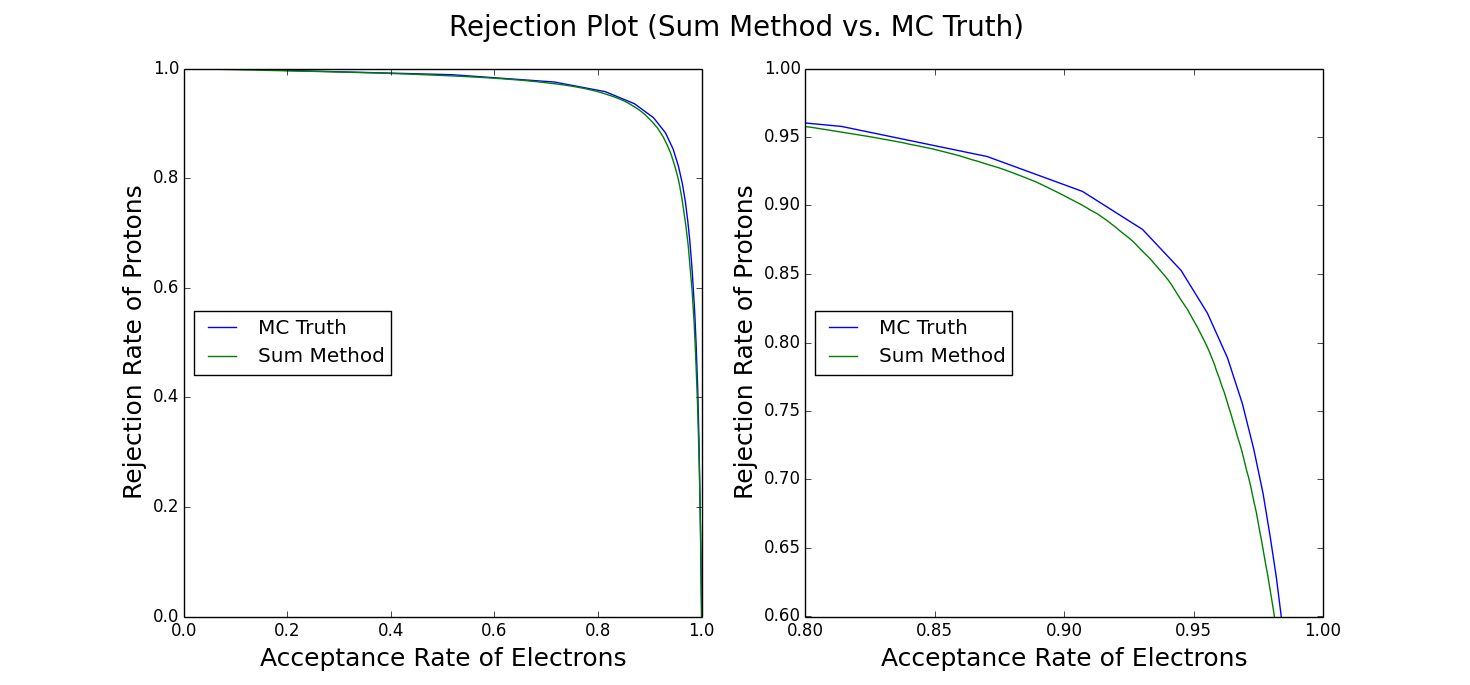
\includegraphics[scale=0.5]{Images2/rejectSumMC.png}}
    \caption{Purity-efficiency curves for sum method and MC energy.}
    \label{rejectionPlotSumAndMCenergy}
\end{figure*} 





\section{Base Fit Method}
 When a particle deposits charge on a straw wire it produces an impulse of current, which is then shaped and digitized by the straw electronics. This shaping can be well-approximated by the composition of an RC and CR filter (Figure \ref{RCCRCircuit}).
%the potential outputted by the ADC would appear as a simple step function. To amplify the signal while controlling the amount of noise a high-pass RC filter followed by a low-pass CR filter have been added to the design. 
\begin{figure}[htp!]
    \centering
    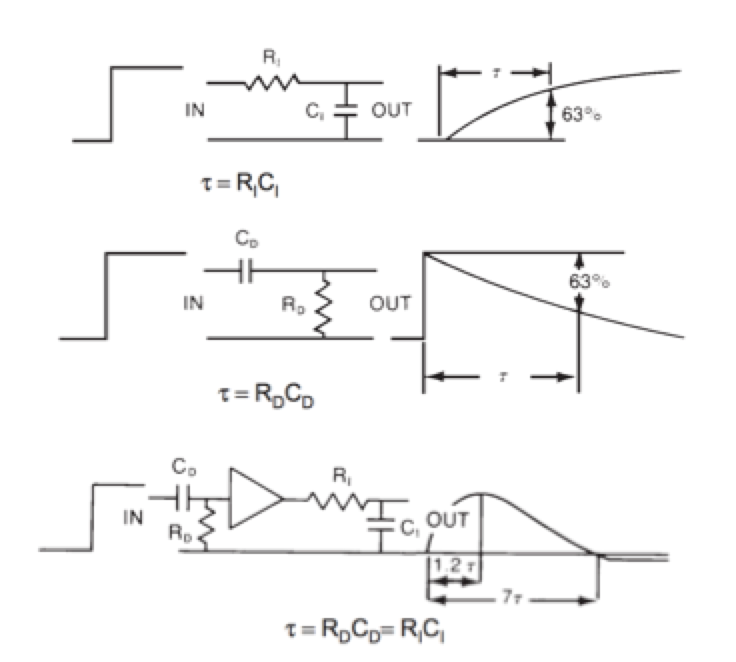
\includegraphics[width=0.6\textwidth]{Images/RCCRCircuit.png}
    \caption{The top diagram shows the effect of an RC circuit on a charge step function, the center shows the effect of a RC circuit on a charge step function, while the bottom diagram depicts the effect of combing these two circuits.}
    \label{RCCRCircuit}
\end{figure} 
This produces a signal of the form 
\begin{equation}
  V(t) = \frac{t}{\tau^2} e^{-t / \tau}
\end{equation}

with shaping time $\tau$.
 For times $t$ less than zero, the function is set to zero.

Qualitatively, most of the hits have this form. However, the waveform can vary in three ways:
\begin{enumerate}
\item The signal's magnitude $(A)$
\item The time at which the signal begins with respect to the 240 ns interval ($t_0$)
\item The initial voltage when the signal begins ($p_0$)
\end{enumerate}
The corresponding functional form is
\begin{equation}
  V(t) = A \frac{(t - t_0)}{\tau^2} e^{-(t - t_0) / \tau} + p_0
  \label{eq:basefit}
\end{equation}.
Note that even though all three of these parameters are necessary to establish the fit, since 
\begin{equation}
  E_{deposited} \propto \int_{0}^{\infty} V(t) - p_0 \text{ } dt = A
\end{equation}
 the energy deposited on the wire is simply proportional to $A$. Hence, after a fit has been applied to a hit, no other computations are necessary to establish the particle's relative energy.

Fitting the ADC data to Equation \ref{eq:basefit}
and extracting the energy from the fit parameter $A$ defines the base fit method. A sample waveform fitted using this method is shown in Figure \ref{fig:sampleBase}.

\begin{figure*}[ht!]
    \centering
    \makebox[0pt]{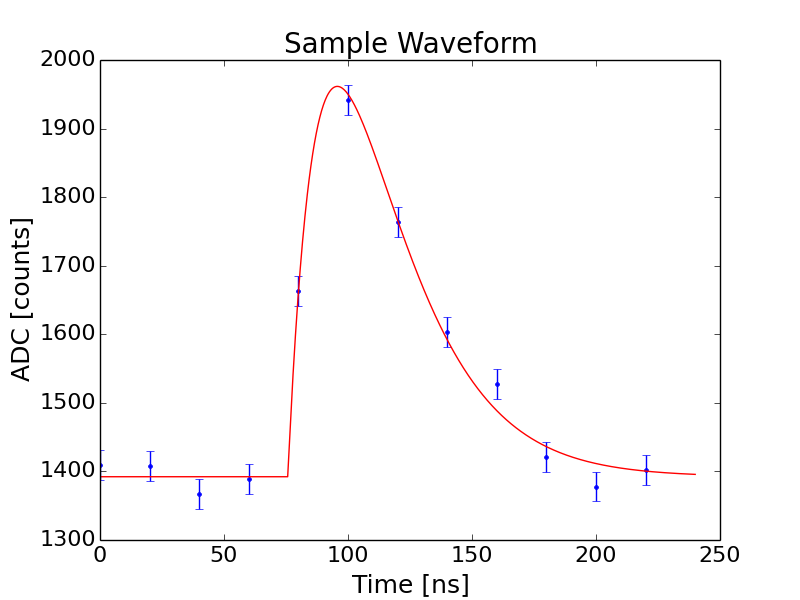
\includegraphics[scale=0.5]{Images2/sampleBase.png}}
    \caption{Sample waveform fitted using basefit method.}
    \label{fig:sampleBase}
\end{figure*} 



%For comparison, consider the plot in Figure \ref{baselineChiSquareDistribution} of the reduced chi-square values of the electron hits fit by this curve. The distribution is centered at one as we would expect. In addition, as shown in Figure \ref{rejectionPlot} this method is better at differentiating electrons and protons than the basic sum method.


%\begin{figure}[htp!]
%    \centering
%    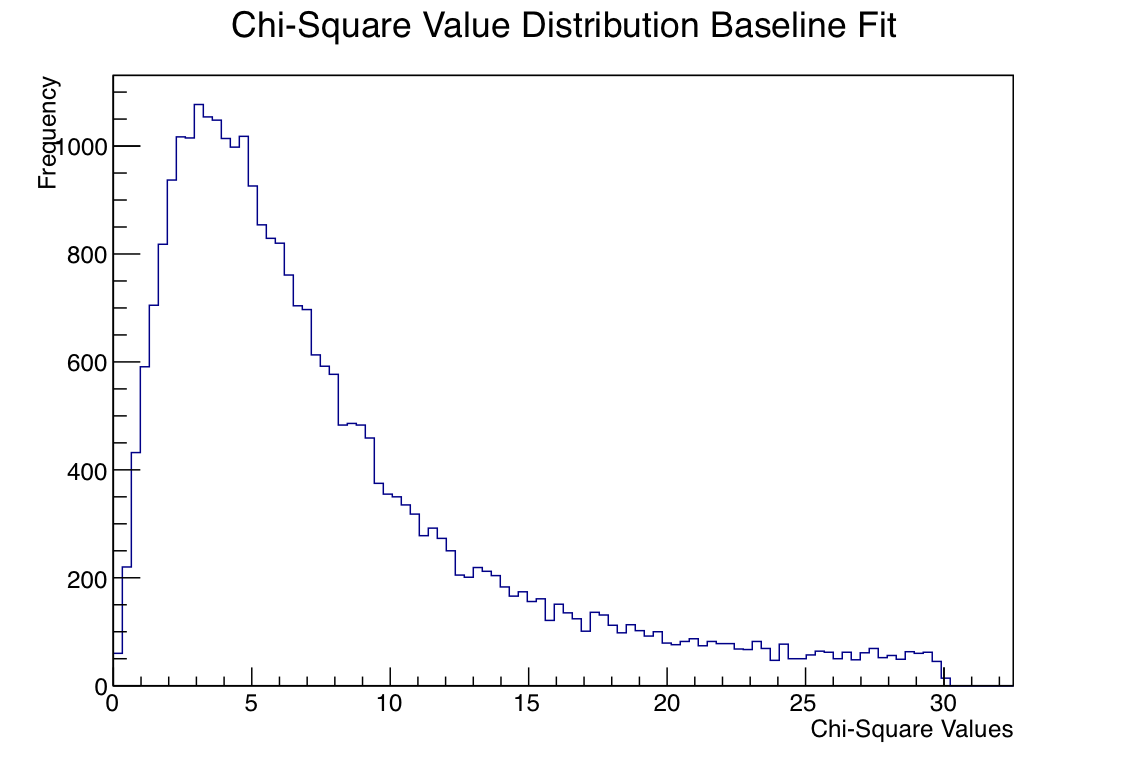
\includegraphics[width=0.6\textwidth]{Images/baselineChisquared.png}
%    \caption{ Chi-squared distributions for the baseline fit method.}
%    \label{baselineChiSquareDistribution}
%\end{figure} 


%For comparison, the reconstructed energies is plotted against the corresponding MC energies. 


%\begin{figure*}[ht!]
%    \centering
%    \makebox[0pt]{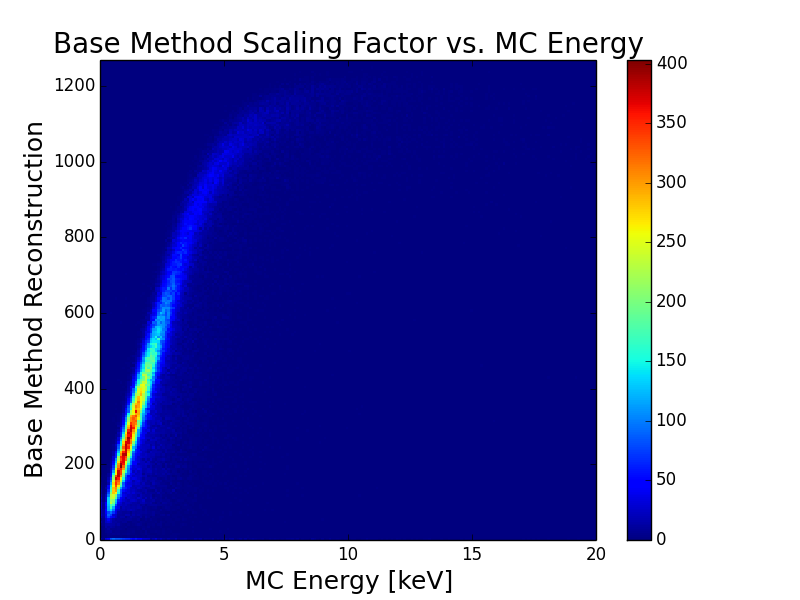
\includegraphics[scale=0.5]{Images2/baseVsMC.png}}
%    \caption{Reconstructed energies using basefit method versus MC energies.}
%    \label{fig:sampleBase}
%\end{figure*} 




For comparison, a frequency plot of the reconstructed energy distributions for the protons and electrons is shown in Figure \ref{fig:recoEnergyFunc1}. From this graph, this fit is quite strong at separating protons and electrons at the 3 KeV energy cut. In addition, it is also apparent that the fit breaks down at higher energies. This is a consequence of saturation in the preamp as discussed Section \ref{sec:preampSaturation}.
 \begin{figure}[htp!]
    \centering
    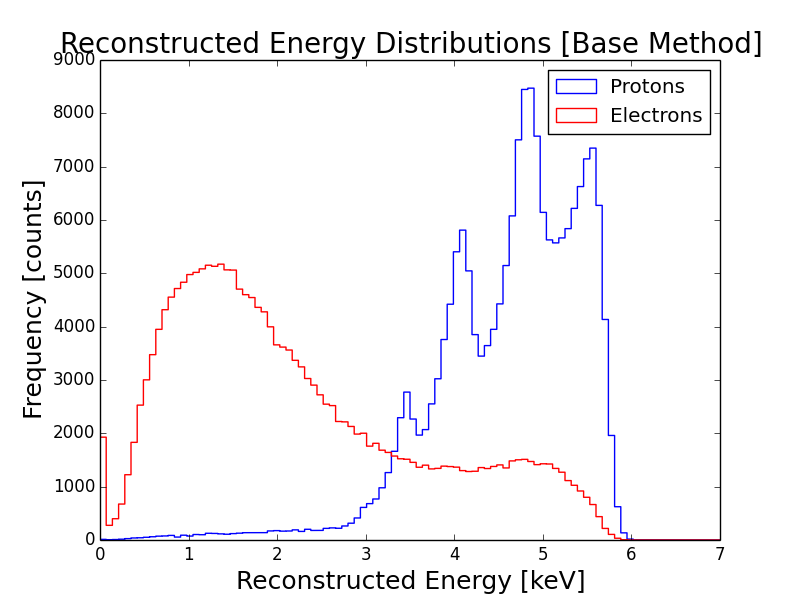
\includegraphics[width=0.6\textwidth]{Images2/base.png}
    \caption{Reconstructed energies using base fit method.}
    \label{fig:recoEnergyFunc1}
\end{figure} 

Clearly, this method is able to differentiate electrons to some degree. However, significant improvements are needed to outperform the sum method. This can be seen from purity-efficiency plot at the end of the chapter.

\section{Convolved Fit Method}
One underlying assumption used in the basefit model is that when a particle passes through a straw it produces a delta function of current on the corresponding wire. However, depending on where in the straw the electron or proton passes the corresponding charge on the wire may be deposited with some spread in time (shown in Figure \ref{fig:hitletTimes}).

\begin{figure}[htp!]
    \centering
    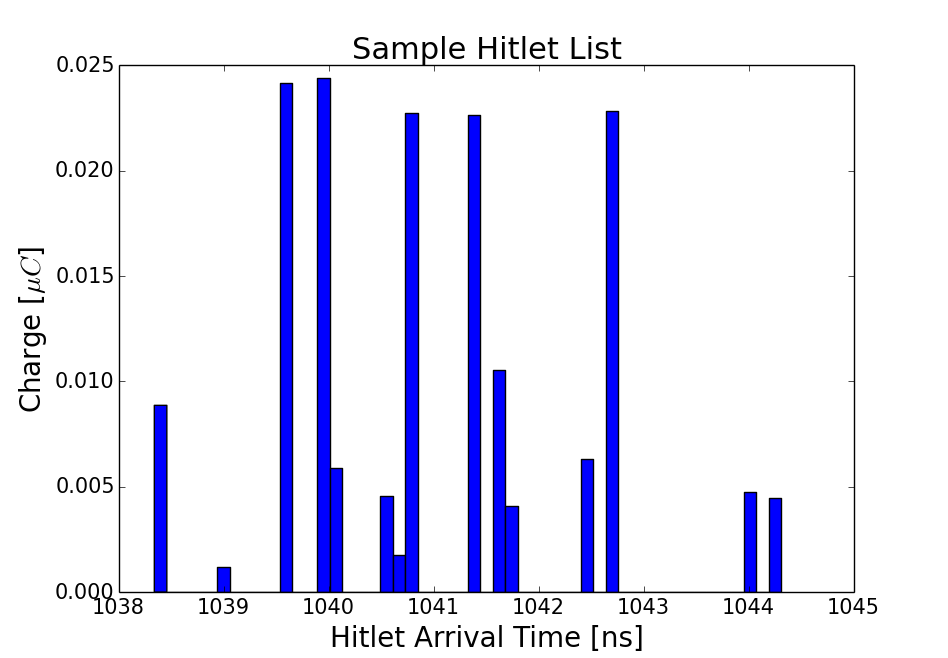
\includegraphics[width=0.6\textwidth]{Images2/hitletlist.png}
    \caption{Simulated arrival times of charges for a given hit.}
    \label{fig:hitletTimes}
\end{figure} 


Consequently, a better approximation for the output from the ADC is the base fit model convolved with a uniform distribution
\begin{equation}
    g(t) = \frac{1}{2 \sigma} \text{ for } t \in \left[ -\sigma, \sigma \right]
\end{equation}
where $\sigma$ is a free parameter defined to be half of the width of the uniform distribution.


Convolving this with Equation \ref{eq:basefit} produces 

\begin{equation}
   V \circ g =  \int_{\infty}^{\infty} V(t - t') g(t') dt' = \left. \frac{1}{2 \sigma}\left[ -e^{-t'} (t' + 1) \right] \right|_{max(\frac{t - \sigma}{\tau},0)}^{max(\frac{t + \sigma}{\tau},0)}
 \end{equation}.

 Adding in $\sigma$ as a free parameter to the fit (in addition to three base  fit parameters), we see that this new fit function is a better fit to the hit in Figure \ref{sampleConvolvedFit}.
 \begin{figure}[htp!]
    \centering
    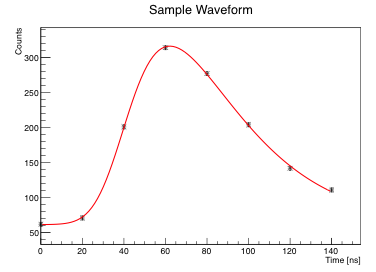
\includegraphics[width=0.5\textwidth]{Images/sampleConvolvedFit.png}
    \caption{Sample waveform with convolved fit.}
    \label{sampleConvolvedFit}
\end{figure} 
 %Consider the following frequency distribution of $\sigma$ from the various fits to events. Although many of the fits lie at $\sigma = 0$ (which is equivalent to the baseline fit model) the majority of fits have values of $\sigma$ greater than $0$, which is indicates that the adding this free parameter is beneficial.

\begin{figure}[htp!]
    \centering
    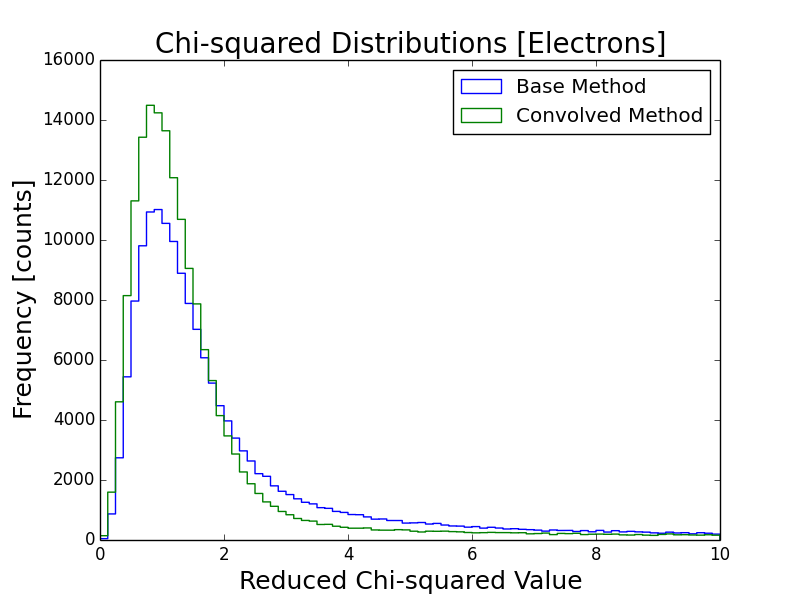
\includegraphics[width=0.6\textwidth]{Images2/chiSquareComparison.png}
    \caption{Chi-square per degree of freedom distributions for the base fit method and convolved fit method.}
    \label{fig:relativeChiSquareDistribution}
\end{figure} 
\begin{figure}[htp!]
    \centering
    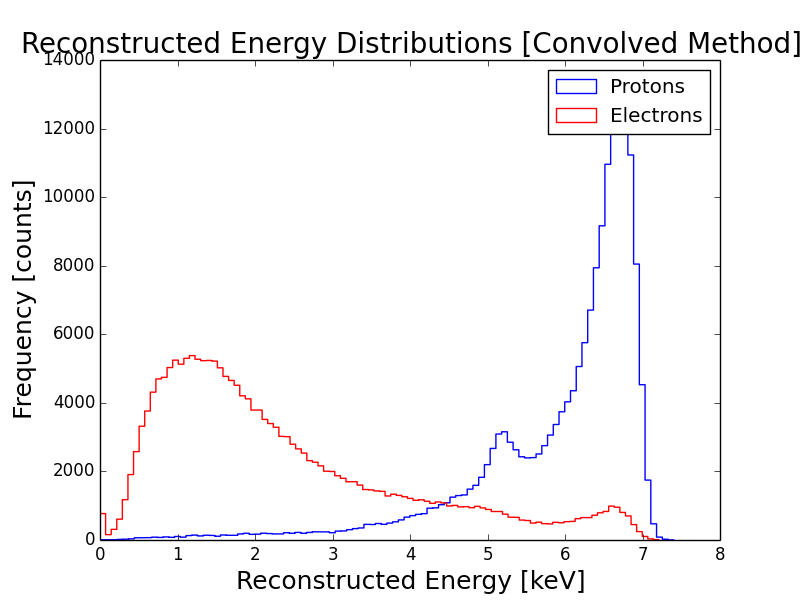
\includegraphics[scale=0.5]{Images2/convolved.png}
    \caption{Reconstructed energies using convolved fit method.}
    \label{recoEnergyFunc6}
\end{figure}


 Figure \ref{fig:relativeChiSquareDistribution} is a plot of the relative chi-squared distributions for the base fit method and the convolved fit method. Clearly, the chi-squared distribution has a much smaller tail and therefore appears to be a more accurate fit for the data.



Like for the base fit method, we can consider a frequency histogram of the reconstructed energies for the electrons and protons (shown in Figure \ref{recoEnergyFunc6}). Differentiation of electrons and protons is somewhat improved for values near 3 keV. However, there is still significant room for improvement, especially at higher energies. 

%However, for very high energies, the reconstructed proton energies appear to have two peaks. Like for the baseline fit, these somewhat unexpected results can be explained by saturation and will be taken into account in the next section.



\section{Fit Method with Saturation \label{sec:sat}}

Consider the plots in Figure \ref{fig:scalingFactVsMCenergy} of the base fit scaling factor versus the MC energy for the proton and electron hits. (Note that the scaling factor has been scaled to a rough estimate of keV.) As predicted, there is a strong linear correlation between the scaling factors and MC energies at lower energies. However, for higher energies the slope clearly begins to flatten.

\begin{figure*}[ht!]
    \centering
    \makebox[0pt]{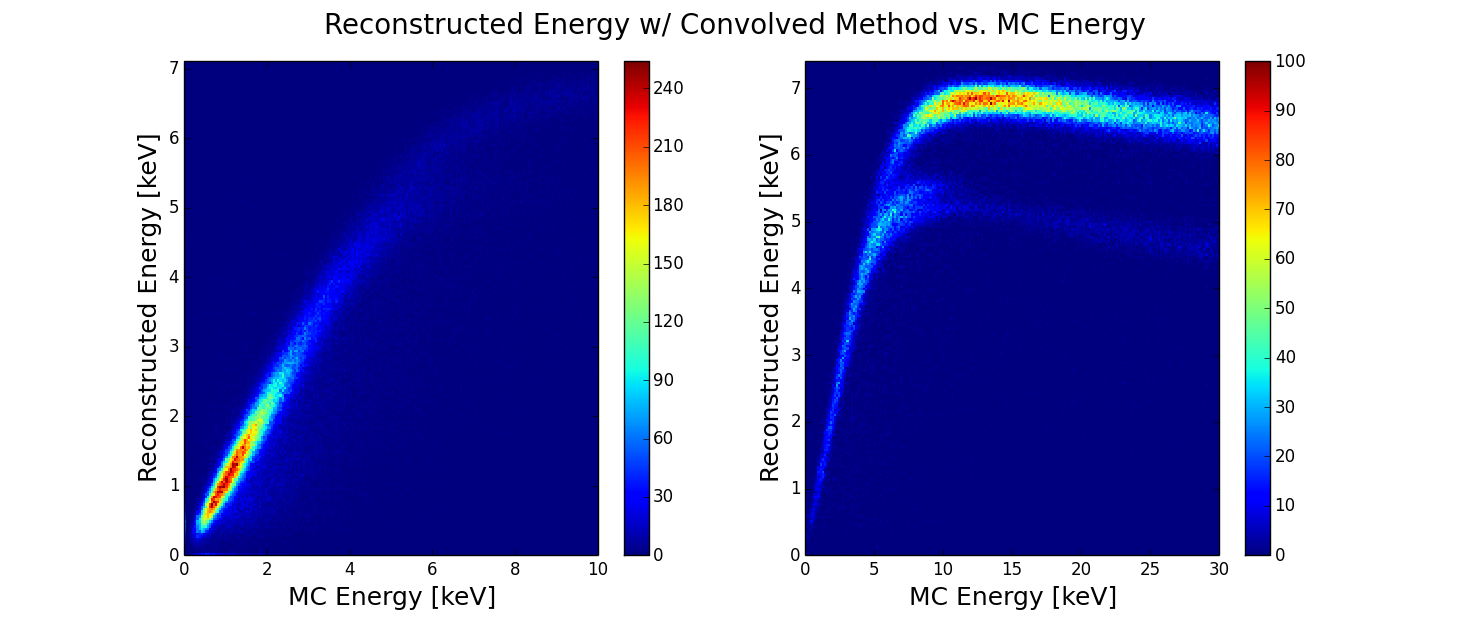
\includegraphics[scale=0.5]{Images2/convolvedVsMC.png}}
    \caption{Computed energy from ADC versus MC energy for electrons (shown on left) and protons (shown on right). Note that the energy from the ADC has been roughly scaled to units of MeV.}
    \label{fig:scalingFactVsMCenergy}
\end{figure*} 

This nonlinearity can easily be attributed to saturation. In particular, this saturation is caused by the preamp in the straws electronics, described in the previous chapter (see Figure ...). 

To improve the energy extraction, the exponential model used to fit the preamp response before, is incorporated into the fit function. The parameters corresponding to the preamp response are known from these previous measurements and thus add no new free parameters to the fit. 
\begin{figure}[htp!]
    \centering
    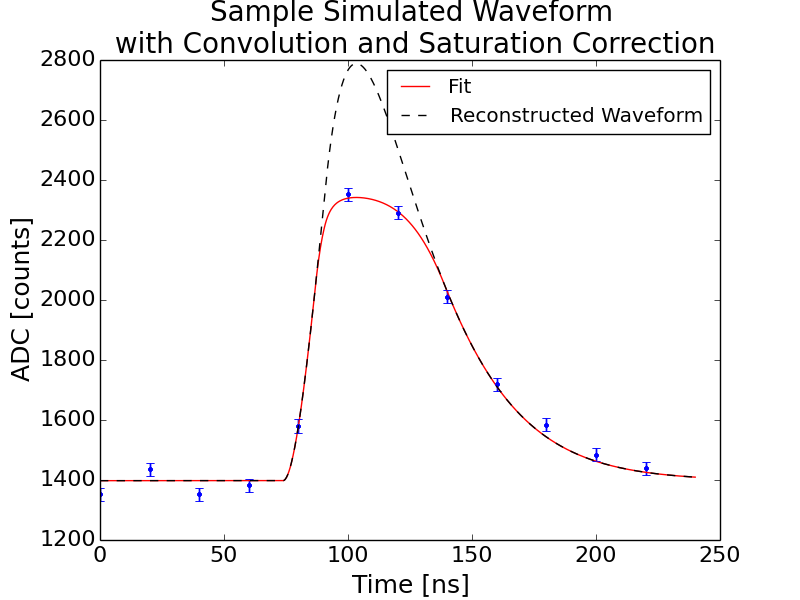
\includegraphics[width=0.5\textwidth]{Images2/recoSat.png}
    \caption{Sample waveform with convolution and saturation correction.}
    \label{fig:recoSat}
\end{figure} 

Figure \ref{fig:recoSat} is a sample waveform in which the fit incorporating saturation is very successful. Figure \ref{protonANDELectronWithTrunction} shows the reconstructed energy using the truncation fit versus the MC energy. Clearly, the response is more linear for both the electrons and protons. Note that although there is spread in the reconstructed energies for high values of MC energies, this spread is in an energy regime far beyond the energy cut value of 3 keV.

\begin{figure}[htp!]
    \centering
    \makebox[0pt]{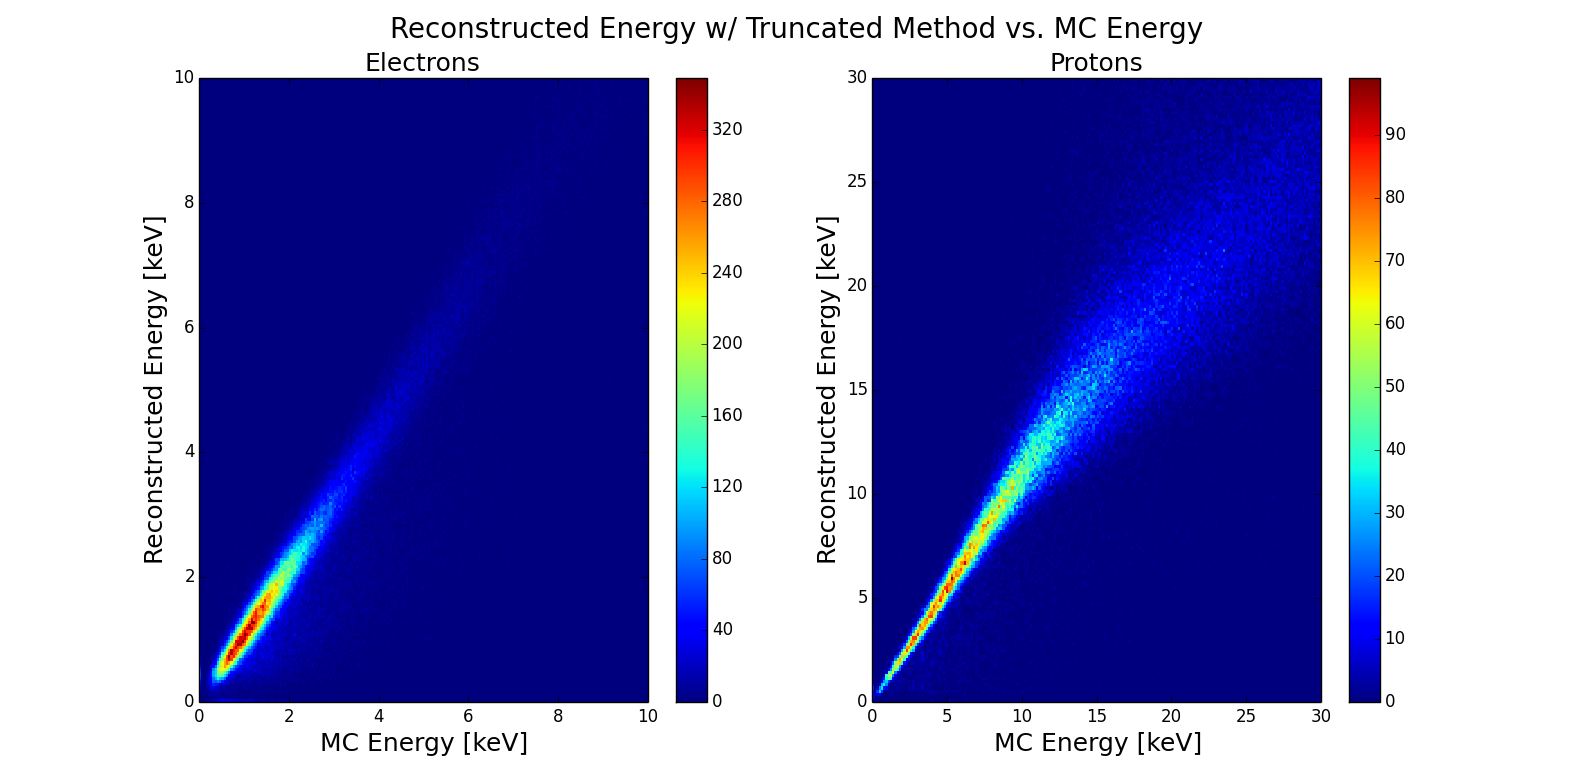
\includegraphics[scale=0.5]{Images2/truncatedVsMC.png}}
    \caption{Reconstructed energies using truncated fit method versus MC energies.}
    \label{protonANDELectronWithTrunction}
\end{figure} 

\begin{figure}[htp!]
    \centering
    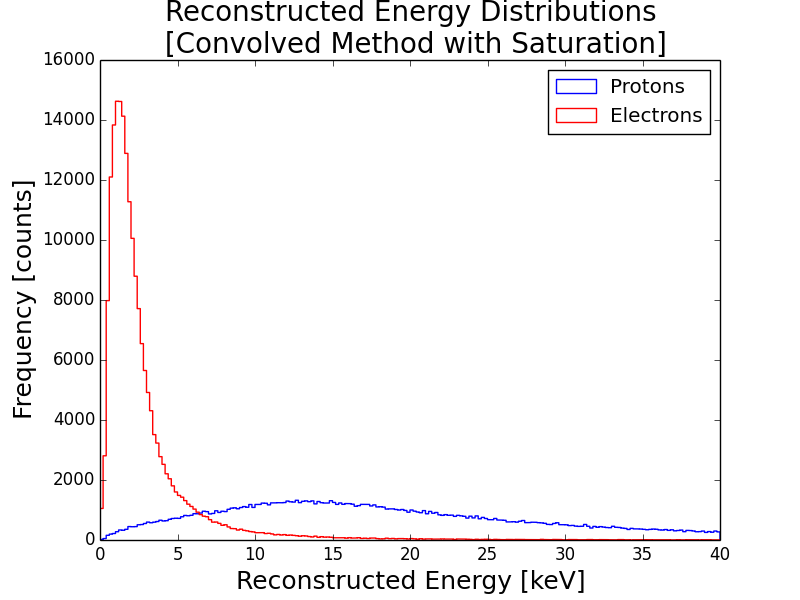
\includegraphics[scale=0.5]{Images2/convolvedSat.png}
    \caption{Reconstructed Energies using truncated fit method.}
    \label{fig:recoEnergyFunc4}
\end{figure} 

This improvement in the fit model can also be seen in the frequency plot of the reconstructed energies (shown in Figure \ref{fig:recoEnergyFunc4}). This is further validated by the corresponding purity-efficiency curve in Figure \ref{fig:rejectionPlot}.

These distributions match those of the corresponding MC energy distribution (Figure \ref{mcenergydistributions}) much more closely than the convolved fit without truncation. In particular, the distributions agree well beyond the 3 keV region, allowing us to recover much of the dynamic range of the ADC. 

In addition, note that this model will be key when fitting cross talk data in which the waveforms will have a similar shape but the reconstructed energies will occur at energies much closer to electrons.
(Should I delete this sentence???)


\section{Multi-peak Methods}
By utilizing the convolution fit method with truncation, the vast majority of data is fit with great accuracy. This final addition, will serve to address a small fraction of hits.


%Consider the frequency histogram (Figure \ref{initialSigmaDistribution}) for the fitting parameter $\sigma$ of the convolved fit. 

%\begin{figure}[htp!]
%    \centering
%    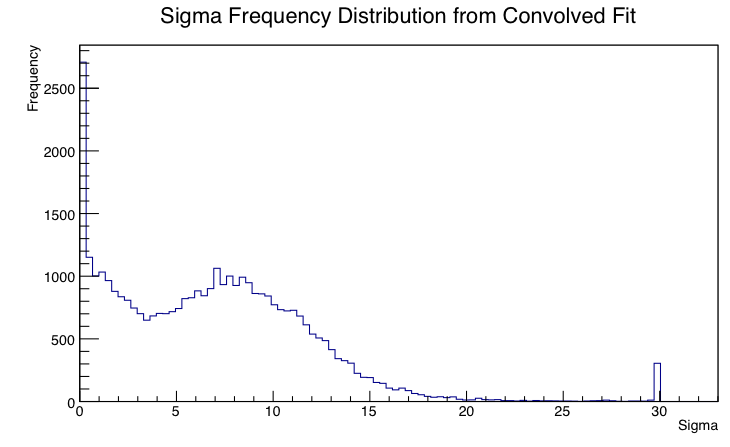
\includegraphics[width=0.7\textwidth]{Images/initialSigmaDistribution.png}
%    \caption{Frequency distribution for the fitting parameter $\sigma$ from the convolved fit.}
%    \label{initialSigmaDistribution}
%\end{figure} 

%It appears that the majority of values are centered around $15$ while falling mainly in the range of $0$ to $25$. In addition, there are two peaks, one at $0$ and one at $30$. The fits with $\sigma = 0$ are fits in which the charge a hit was deposited on the wire approximately instantaneously. Therefore, this peak is physically meaningful and warrants no concern. The peak at $\sigma = 30$ is a consequence of the fact that a limit of $30$ was placed on the fit parameter. Consequently, this peak actually corresponds to a tail reaching beyond $30$, and upon inspection consists of poor fits.




For many of these fits the output appears to be a superposition of multiple waveforms occuring within the same 240 ns period. To further explore this an explicit peak search was applied to the data. A distribution of the number of peaks found is shown in Figure \ref{fig:peakSearch}. From this figure, we can see that roughly five percent of hits recorded contain more than one peak. Two methods are used to address this possibility.

\begin{figure}[htp!]
    \centering
    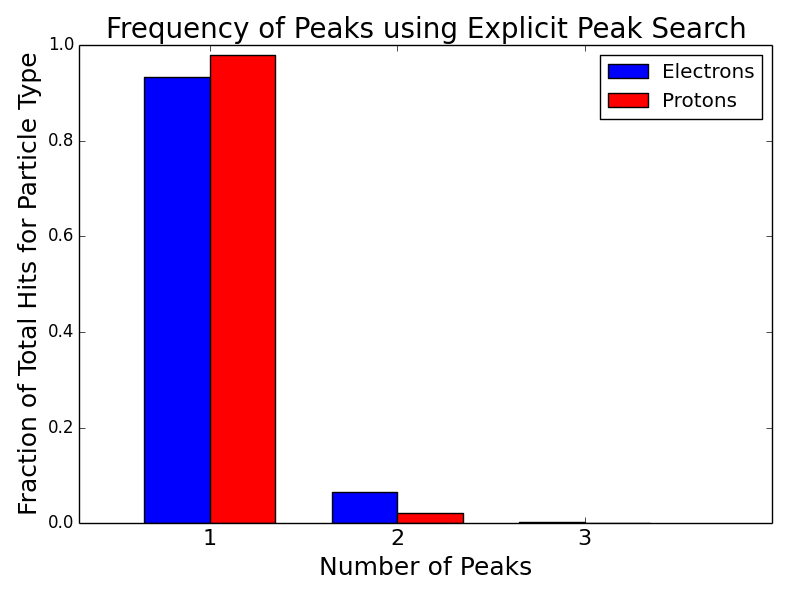
\includegraphics[width=0.7\textwidth]{Images2/peakSearch.png}
    \caption{Distribution of peaks found using explicit peak search.}
    \label{fig:peakSearch}
\end{figure} 


\subsection{Early Peak Method}

 One possibility for a double peak hit is that the primary hit for the 240 ns period is superimposed on a previous waveform which has not sufficiently decayed. Since the end of a waveform can be well-approximated by an exponential decay, a term of the form $Q(t) = e^{-t / \tau}$ can be added to the fit function. A sample fit is shown in Figure \ref{fig:earlyPeak}.

  %This additional approximately exponential decay, can force the fitted value of the pedestal to be overestimated which results in a event which can not be well-fitted by a simple convoluted fit. To address this issue an approximate solution to the decay of a waveform $Q(t) = e^{-t / \tau}$ can be added to the fit function. 
  %As can be seen in the sample fit, this solution appears to be succesful, and reduces several of the high sigma values.  

\begin{figure}[htp!]
    \centering
    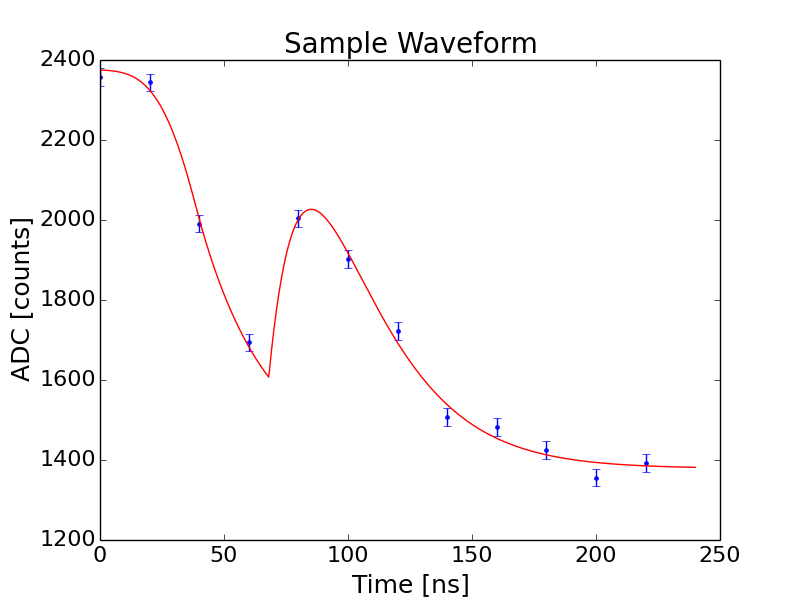
\includegraphics[scale=0.6]{Images2/dynamicPed.png}
    \caption{Sample waveform fitted with early peak method.}
    \label{fig:earlyPeak}
\end{figure} 
%A plot of the reconstructed energies for the protons and electrons is shown in Figure \ref{recoEnergyFunc7}. Note that there is not a significant change in the distributions with respect to the corresponding plot using the truncated fit method.



\subsection{Late Peak Method}

A double peak hit can also occur when a secondary hit occurs shortly after the primary hit. To model this, two of the base convolved fits can be summed together. To speed up the fitting process and to control the complexity of the fit model, the convolution parameter of $\sigma$ for both hits are fixed to $7$ ns. Thus, there are five free parameters in the fit. Note that the value of $7$ is fairly arbitrary, but has been found to be fairly reasonable. (Should I refer to sigma distribution here?)


%To reduce the number of free parameters



%Note that we cannot use two convolved fits, since we do not have enough information for each hit ($8$ samples - $8$ fit parameters = $0$ degrees of freedom). In addition, note that by using the baseline fit, we have assumed a value of $\sigma = 0$ for each peak. However, from \ref{initialSigmaDistribution} another option might be to use two convolved fits with $\sigma$ fixed to 8.

%Adjusting the fit parameters so that the two peaks can not overlap significantly, we are able to achieve a relatively successful fit. Note that this fit is only successful for fits which contain two peaks. Therefore, its use must be restricted to certain cases. Hence, this fit is only effective when used alongside the convolved fit with a dynamic pedestal. 

\begin{figure}[htp!]
    \centering
    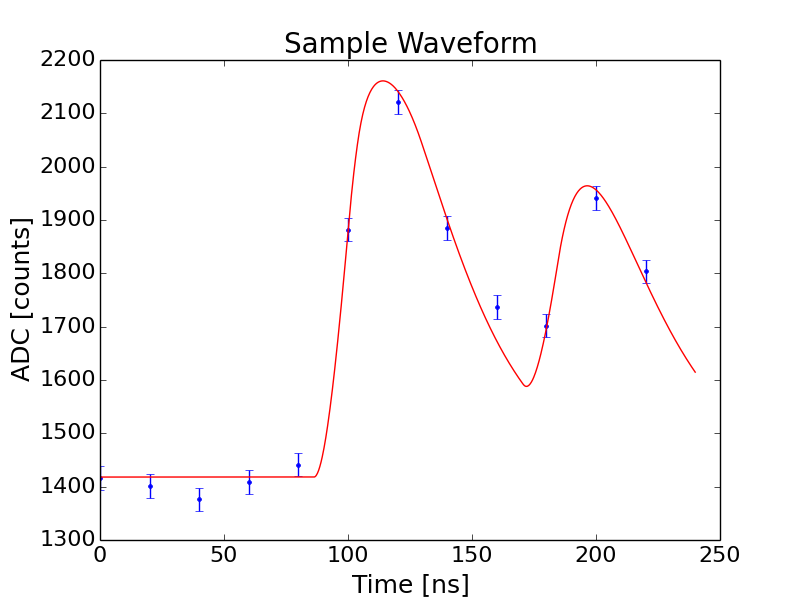
\includegraphics[width=0.6\textwidth]{Images2/double.png}
    \caption{Sample waveform fitted with late peak method.}
\end{figure} 

\begin{figure}[htp!]
    \centering
    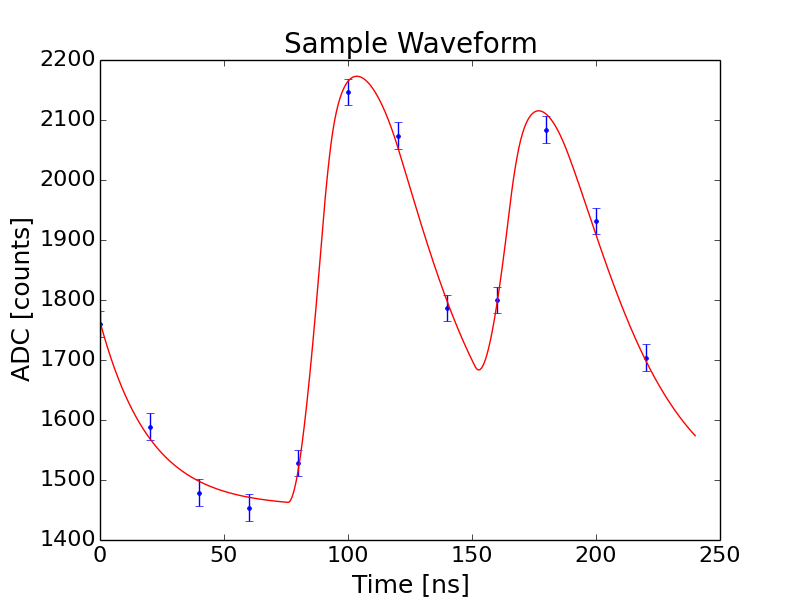
\includegraphics[width=0.6\textwidth]{Images2/full.png}
    \caption{Sample fit with both an early peak and a late peak.}
    \label{fig:full}
\end{figure} 

\subsection{Early and Late Peak Method}
For completion, note that in Figure \ref{fig:peakSearch}, there are a small subset of hits in which three peaks are found. These cases can be fit to a model which contains both an early and a late peak. A sample fit is shown in Figure \ref{fig:full}.



\subsection{Triage Method}
In summary, by first applying an explicit peak search, 
we can determine the number and approximate locations of peaks over for each given 240 ns interval. With this information, we can determine whether to use a convolved fit or a multi-peak fit method. Note that determining whether the secondary peak is an early peak is extremely simple : simply 

%To determine whether to use the double peak fit method or the convolved fit method with the dynamic pedestal the following algorithm has been used: if the chisquare value from the dynamic pedestal method is at least three times greater than the chisquare value for the double peak fit method, use the dynamic pedestal method. Otherwise, use the double peak fit method. Note that this algorithm for differentiating the waveforms has not yet been optimized.

Using this algorithm, energy distributions for electrons and protons can be reproduced (Figure ). Note that this plot closely resembles Figure \ref{fig:recoEnergyFunc4} since the addition of the triage only effects the analysis of roughly 5 percent of hits.

\begin{figure}[htp!]
    \centering
    \makebox[0pt]{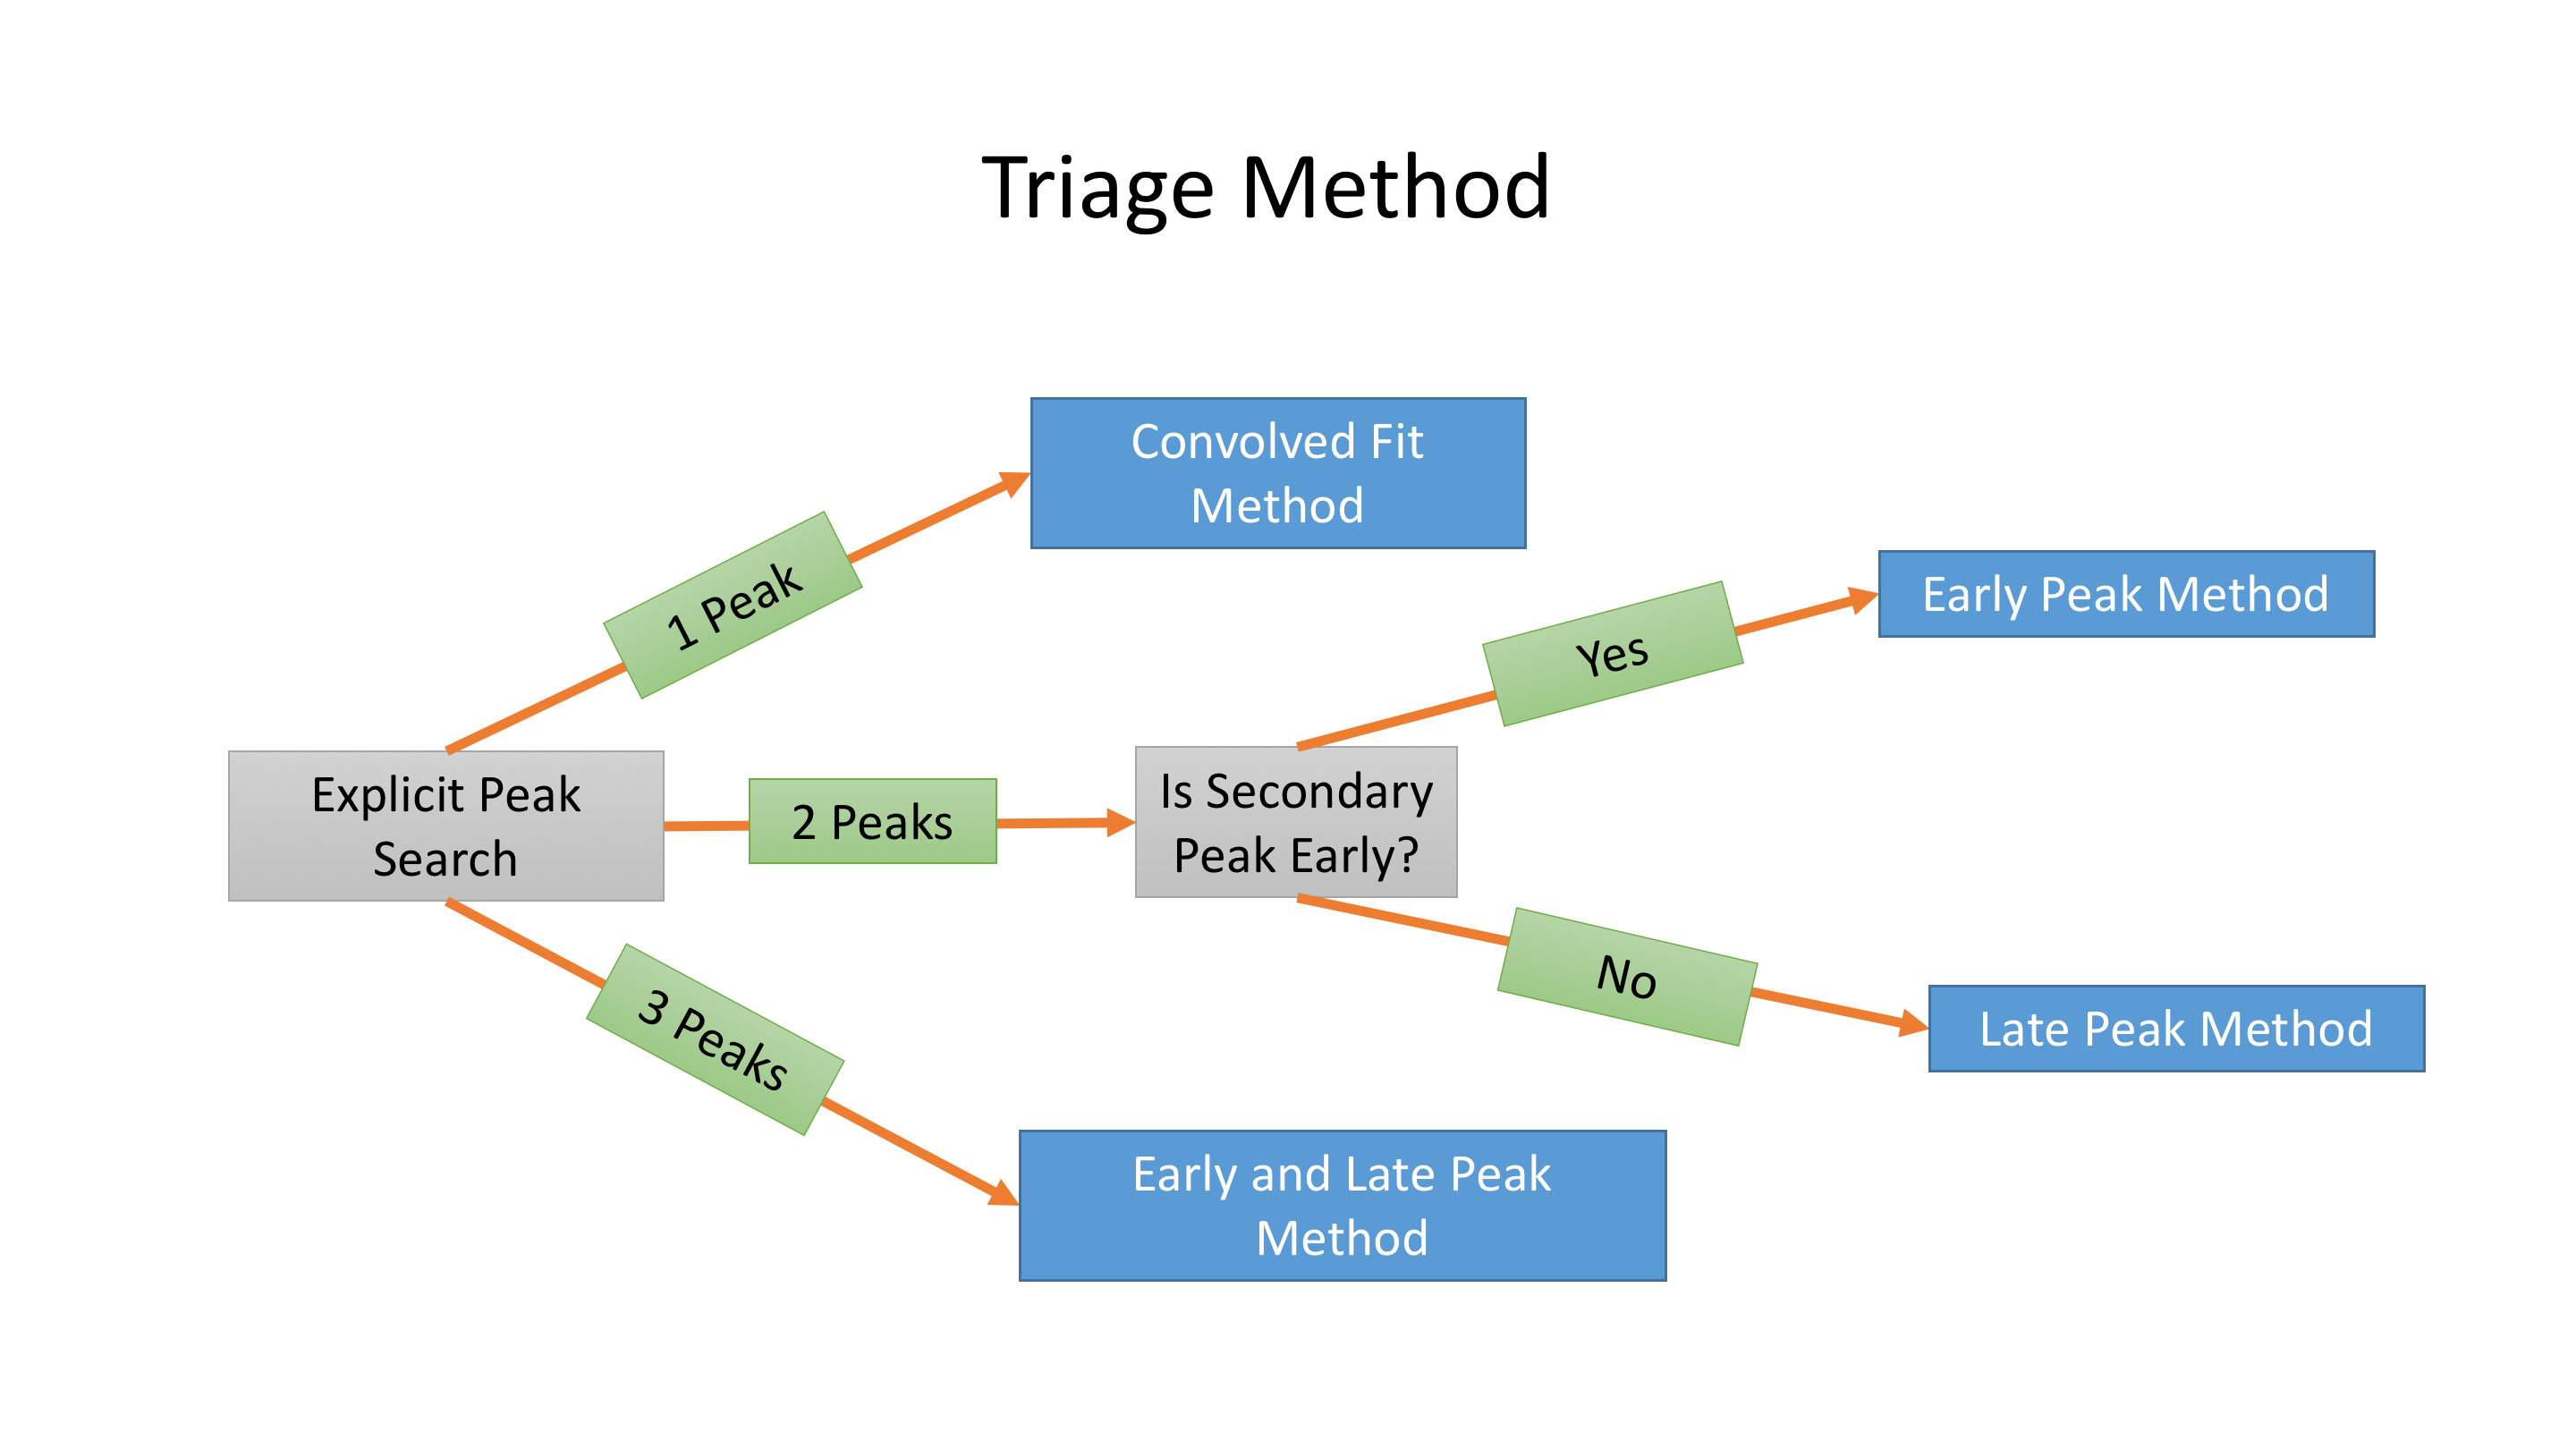
\includegraphics[scale=0.4]{Images2/triageMethod.png}}
    \caption{Decision processes used in triage method.}
    \label{fig:triage}
\end{figure} 



\begin{figure}[htp!]
    \centering
    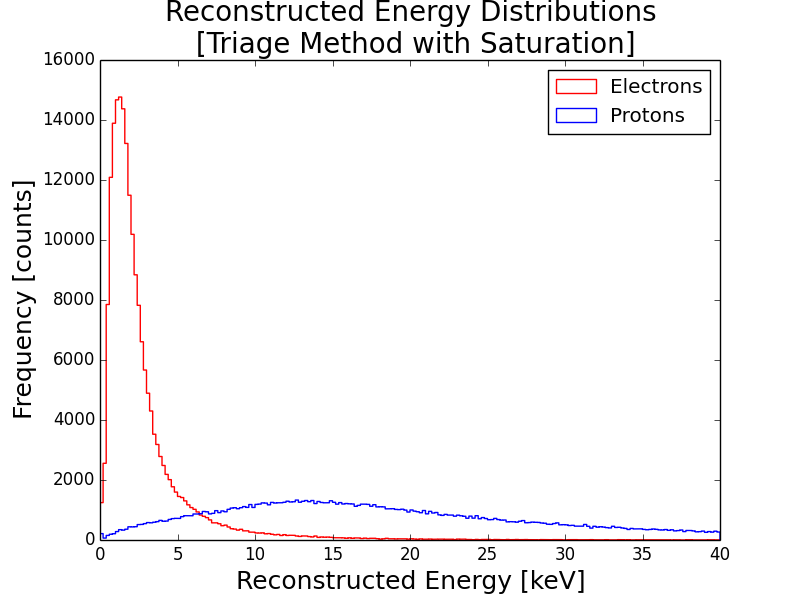
\includegraphics[width=0.6\textwidth]{Images2/triage.png}
    \caption{Reconstructed Energies using triage method with truncation.}
    \label{fig:triage}
\end{figure} 

%After utilizing this algorithm, the distribution of the parameter $\sigma$ has been reproduced (Figure \ref{finalSigmaDistribution}). Note that, all fits corresponding to double peaks (as determined from the algorithm in the previous paragraph) have been removed. 
%\begin{figure}[htp!]
%    \centering
%    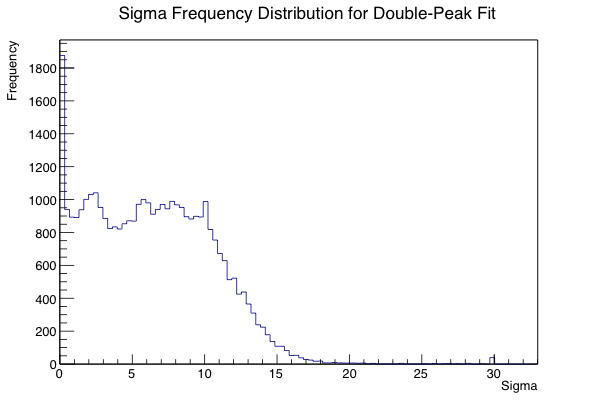
\includegraphics[width=0.55\textwidth]{Images/finalSigmaDistribution.png}
%    \caption{Computed energy from ADC versus MC energy. Note that the energy from the ADC has been roughly scaled to units of MeV.}
%    \label{finalSigmaDistribution}
%\end{figure} 

%Clearly, this method is successful in eliminating the tail in the sigma distribution.

%Lastly, for comparison consider the frequency plot of the reconstructed energies of the protons and electrons (Figure \ref{recoEnergyFunc8}). No significant changes can be seen in the distributions for the two particles.


\begin{figure}[htp!]
    \centering
    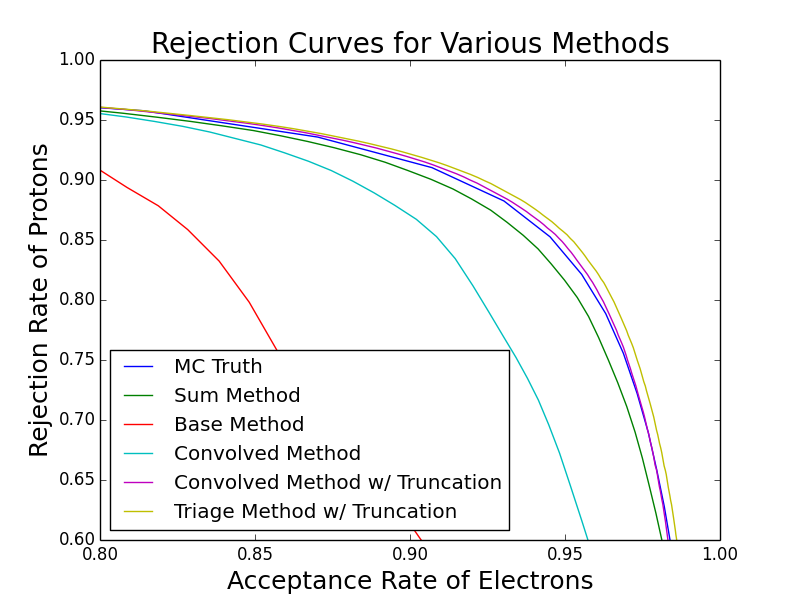
\includegraphics[scale=0.6]{Images2/rejectAll.png}
    \caption{Reconstructed Energies using triage method with truncation.}
    \label{fig:rejectionPlot}
\end{figure} 


\section{Results} 

As described at the beginning of this chapter, the figure of merit is the comparison of the rejection curves for the various methods, which is presented in Figure \ref{fig:rejectionPlot}.

The base fit method and convolved fit methods perform worse than the sum method. However, by introducing the convolved and saturation models, the fit method performs significantly better. In fact, it performs better than differentiation using the MC energy. This makes sense, since even without triage, the convolved fit method will sometimes fit to the primary peak even if other peaks appear in the waveform.

Lastly, it is clear that the triage method performs the best.  In the range relevant to the Mu2e experiment (which corresponds to an approximately a 95\% acceptance rate of electrons), the triage fit method has rejects over 22 percent of proton hits accepted by the sum method.

 %approximately an 1\% improvement over the sum method. In particular, the double peak method performs the best as it can differentiate double particles while the MC energy can not. Note that the double peak fit method will likely perform better in the actual experiment, since less double peak hits appeared in the data used than would be expected. (This is a result of a compromise made in order to measure more high energy electron hits. This effect will be removed in future studies.)



 %\[ f(v_{in}) =  \left\{
 %       \begin{array}{ll}
 %           v_{in} & \quad v_{in} \leq v_{sat} \\
 %           v_{max} - (v_{max} - v_{sat}) e^{-\frac{v_{in} - v_{sat}}{v_{max} - v_{sat}}} & \quad v_{in} > v_{sat}
  %      \end{array}
  %  \right.
%\] 


